% Общий вид транспортной таблицы: строки — пункты хранения A_i с запасами a_i,
% столбцы — пункты назначения B_j с потребностями b_j, в клетках тарифы c_ij.
\begin{figure}[htbp]
\centering
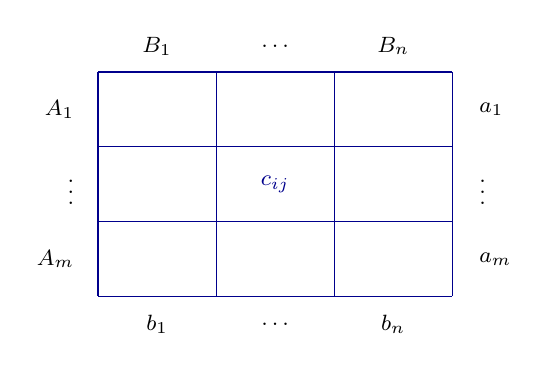
\begin{tikzpicture}[scale=1.0]

\def\cw{1.5}   % ширина клетки
\def\ch{0.95}  % высота клетки

% сетка 3 x 3 (схематично: первая строка, многоточие, последняя строка)
\foreach \i in {0,1,2,3}
  \draw[blue!55!black] (0, -\i*\ch) -- (3*\cw, -\i*\ch);
\foreach \j in {0,1,2,3}
  \draw[blue!55!black] (\j*\cw, 0) -- (\j*\cw, -3*\ch);

% заголовки столбцов
\node[font=\footnotesize] at (0.5*\cw,  0.33) {$B_1$};
\node[font=\footnotesize] at (1.5*\cw,  0.33) {$\dots$};
\node[font=\footnotesize] at (2.5*\cw,  0.33) {$B_n$};

% заголовки строк
\node[font=\footnotesize, anchor=east] at (-0.18, -0.5*\ch) {$A_1$};
\node[font=\footnotesize, anchor=east] at (-0.18, -1.5*\ch) {$\vdots$};
\node[font=\footnotesize, anchor=east] at (-0.18, -2.5*\ch) {$A_m$};

% запасы справа
\node[font=\footnotesize, anchor=west] at (3*\cw+0.22, -0.5*\ch) {$a_1$};
\node[font=\footnotesize, anchor=west] at (3*\cw+0.22, -1.5*\ch) {$\vdots$};
\node[font=\footnotesize, anchor=west] at (3*\cw+0.22, -2.5*\ch) {$a_m$};

% потребности снизу
\node[font=\footnotesize] at (0.5*\cw, -3*\ch-0.35) {$b_1$};
\node[font=\footnotesize] at (1.5*\cw, -3*\ch-0.35) {$\dots$};
\node[font=\footnotesize] at (2.5*\cw, -3*\ch-0.35) {$b_n$};

% тарифы в центре
\node[font=\footnotesize, blue!55!black] at (1.5*\cw, -1.5*\ch) {$c_{ij}$};

\end{tikzpicture}
\caption{Транспортная таблица. Строки — пункты хранения $A_i$ с запасами $a_i$,
столбцы — пункты назначения $B_j$ с потребностями $b_j$, в клетке $(i,j)$ стоит
тариф $c_{ij}$, а при заполнении плана — ещё и объём перевозки $x_{ij}$.}
\label{fig:transport-table}
\end{figure}
